\documentclass[a4paper,10pt]{article}
\usepackage{graphicx}
\usepackage[russian]{babel}
\usepackage{cmap}
\usepackage[T2A]{fontenc}
\usepackage[utf8]{inputenc}
\usepackage{mathtools}
\usepackage{float}
\usepackage{titlesec}
\usepackage{varioref}
\usepackage{fancyhdr}
\usepackage{multicol}
\usepackage{mathrsfs}
\usepackage{wrapfig}
\usepackage{gensymb}
\usepackage{subcaption}         
\usepackage[table,xcdraw]{xcolor}



\begin{document}

	
    
	\begin{center}
		{\large МОСКОВСКИЙ ФИЗИКО-ТЕХНИЧЕСКИЙ ИНСТИТУТ (НАЦИОНАЛЬНЫЙ ИССЛЕДОВАТЕЛЬСКИЙ УНИВЕРСИТЕТ)}
		\end{center}
		
		
		
	\vspace{4.5cm}
		{\Large
	\begin{center}
	\end{center}
				{\bf Отчёт о выполнении лабораторной работы 3.4.2}\\
				Закон Кюри-Вейсса
		}
	\vspace{2cm}
		\begin{flushright}
			{\normalsize Галкина Мария, Высоцкая Ирина \\
				\vspace{0.2cm}
				Б03-502}
		\end{flushright}
		\vspace{8cm}
		

\section{Аннотация}
\noindent \textbf{Цель работы:} изучение температурной зависимости магнитной восприимчивости ферромагнетика выше точки Кюри\\
\textbf{В работе используются:} катушка самоиндукции с образцом из гадолиния, теромстат, цифровой вольтметр, LC-автогенератор, термопара медь-константан.

\section{Теоретические сведения}


Вещества, атомы которых обладают отличным от нуля магнитным моментом, называются \textbf{парамагнетиками}. В отсутствие внешнего магнитного поля эти моменты расположены в пространстве хаотично из-за теплового движения. При внесении во внешнее магнитное поле оно стремится ориентировать магнитные моменты вдоль поля, создавая намагниченность. При повышении температуры \(T\) возрастает дезориентирующее действие теплового движения, и магнитная восприимчивость парамагнетиков уменьшается обратно пропорционально температуре (закон Кюри):
\begin{equation}
    \chi \propto \frac{1}{T}.
\end{equation}

Некоторые парамагнетики при понижении температуры испытывают фазовый переход в \textbf{ферромагнитное состояние}. В этом состоянии благодаря обменному взаимодействию (имеющему электростатическую природу) возникает самопроизвольное упорядочение магнитных моментов атомов в одном направлении даже при сколь угодно слабом внешнем поле. Температура, при которой происходит фазовый переход парамагнетик--ферромагнетик, называется \textbf{температурой (точкой) Кюри} \(\Theta_K\).

При температурах выше точки Кюри (\(T > \Theta_K\)) тепловое движение разрушает дальний магнитный порядок. В этой области температурная зависимость магнитной восприимчивости ферромагнетика с удовлетворительной точностью описывается \textbf{законом Кюри--Вейсса}:
\begin{equation}
    \chi \propto \frac{1}{T - \Theta_p},
\end{equation}
где \(\Theta_p\) — параметр с размерностью температуры, называемый \textit{парамагнитной точкой Кюри}. Величина \(\Theta_p\) близка к \(\Theta_K\), но не совпадает с ней. Непосредственно вблизи \(\Theta_K\) закон Кюри--Вейсса нарушается.

\subsection*{Метод измерения магнитной восприимчивости}

В работе исследуется зависимость \(\chi(T)\) гадолиния. Образец ферромагнетика помещается внутрь катушки самоиндукции, которая является индуктивностью \(LC\)-автогенератора. Коэффициент самоиндукции катушки пропорционален магнитной проницаемости \(\mu\) заполняющей её среды: \(L \propto \mu\). Следовательно, разность индуктивностей катушки с образцом и без него пропорциональна магнитной восприимчивости:
\begin{equation}
    L - L_0 \propto \mu - 1 = \chi.
\end{equation}

Период колебаний равен \(\tau = 2\pi\sqrt{LC}\). Период колебаний в отсутствие образца: \(\tau_0 = 2\pi\sqrt{L_0 C}\). Отсюда разность индуктивностей выражается через квадраты периодов:
\begin{equation}
    L - L_0 \propto \tau^2 - \tau_0^2.
\end{equation}

Следовательно, магнитная восприимчивость образца пропорциональна разности квадратов периодов:
\begin{equation}
    \chi \propto \tau^2 - \tau_0^2.
\end{equation}

Из совместного решения уравнений (2) и (5) следует, что закон Кюри--Вейсса справедлив, если выполнено соотношение:
\begin{equation}
    \frac{1}{\tau^2 - \tau_0^2} \propto T - \Theta_p.
\end{equation}
Таким образом, график зависимости \(1/(\tau^2 - \tau_0^2)\) от температуры \(T\) должен представлять собой прямую линию, экстраполяция которой к оси абсцисс дает значение парамагнитной точки Кюри \(\Theta_p\).




\section{Экспериментальные данные и обработка результатов}

\subsection*{Расчет допустимой ЭДС термопары}
Согласно заданию, оценим допустимую ЭДС термопары, если допустимая разность температур образца и рабочей жидкости \(\Delta T = 0.5^\circ\text{C}\), а температурный коэффициент термопары \(\alpha = 24 \text{ град/мВ}\).
\[
U_{\text{доп}} = \frac{\Delta T}{\alpha}  \approx 20.8 \text{ мкВ}.
\]

\subsection*{Расчет температуры образца и построение графика}
Температура образца \(T\) рассчитывалась с учетом показаний термопары \(\Delta U\):
\[
T = T_{\text{терм}} + \alpha \cdot \Delta U,
\]
где знак ``\(+\)'' берется, если температура образца выше температуры рабочей жидкости.

Величина \(1/(\tau^2 - \tau_0^2)\) рассчитывалась на основе измеренного периода колебаний \(\tau\) и периода без образца \(\tau_0 = 9.045 \text{ мкс}\).

Результаты измерений и расчетов представлены в таблице~\ref{tab:data}.

\begin{table}[H]
\centering
\caption{Результаты измерений и расчетов}
\label{tab:data}
\begin{tabular}{|c|c|c|c|c|}
\hline
\(T_{\text{терм}}, ^\circ\text{C}\) & \(\Delta U, \text{мВ}\) & \(T, ^\circ\text{C}\) & \(\tau, \text{мкс}\) & \(1/(\tau^2-\tau_0^2), \text{мкс}^{-2}\) \\
\hline
14.12 & -0.0010 & 14.10 & 10.7800 & 0.0276 \\
16.00 & -0.0090 & 15.78 & 10.7180 & 0.0280 \\
18.02 & -0.0060 & 17.88 & 10.5440 & 0.0331 \\
20.03 & -0.0027 & 19.97 & 10.2180 & 0.0442 \\
22.00 & -0.0060 & 21.86 & 9.9220 & 0.0598 \\
24.00 & -0.0088 & 23.79 & 9.6000 & 0.0953 \\
26.01 & -0.0030 & 25.94 & 9.4260 & 0.1413 \\
28.00 & -0.0088 & 27.79 & 9.3580 & 0.1683 \\
30.00 & -0.0780 & 28.13 & 9.3036 & 0.2098 \\
32.00 & -0.0083 & 31.80 & 9.2720 & 0.2407 \\
34.00 & -0.0059 & 33.86 & 9.2430 & 0.2706 \\
36.00 & -0.0078 & 35.81 & 9.2260 & 0.3015 \\
38.00 & -0.0076 & 37.82 & 9.2110 & 0.3275 \\
40.00 & -0.0089 & 39.79 & 9.1990 & 0.3551 \\
\hline
\end{tabular}
\end{table}

На рисунке~\ref{fig:graph} представлена зависимость \(1/(\tau^2 - \tau_0^2) = f(T)\). 
\begin{figure}[H]
\centering
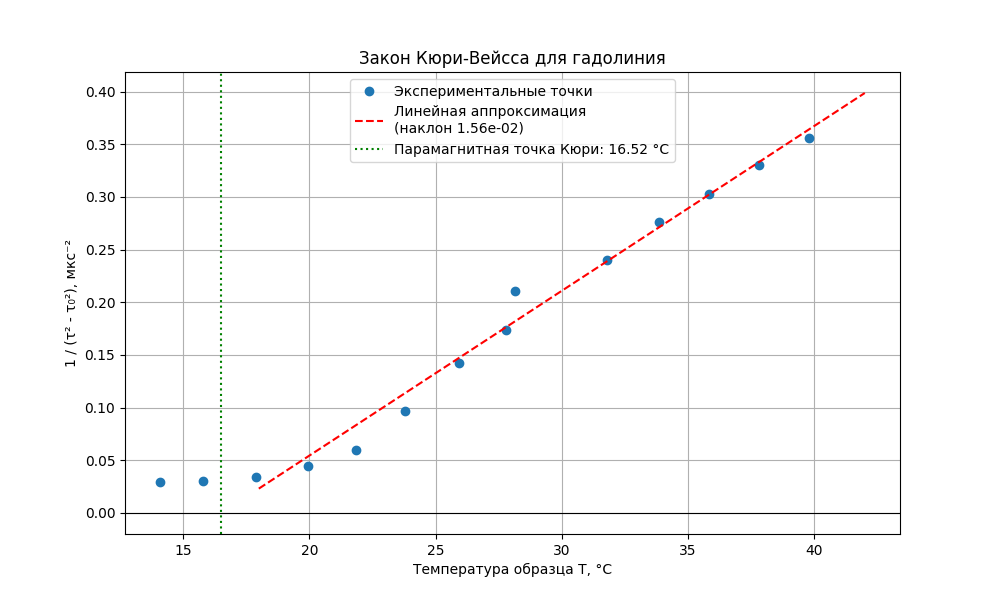
\includegraphics[width=1\textwidth]{график.png}
\caption{Зависимость обратной величины магнитной восприимчивости от температуры}
\label{fig:graph}
\end{figure}

\subsection*{Определение точек Кюри}
Экстраполируя линейный участок графика (для температур \(T > 22^\circ\text{C}\)) к оси абсцисс, находим \textbf{парамагнитную точку Кюри}:
\[
\Theta_p \approx 16.5 ^\circ\text{C}.
\]

По участку, отклоняющемуся от линейной зависимости (при \(T < 22^\circ\text{C}\)), оценим положение \textbf{ферромагнитной точки Кюри} \(\Theta_K\). Отклонение от закона Кюри--Вейсса начинается примерно при \(T \approx 20 \dots 22 ^\circ\text{C}\), что соответствует \(\Theta_K \approx 20 ^\circ\text{C}\).



\subsection*{Определение точек Кюри (с исключением выброса)}
При обработке данных было замечено, что экспериментальная точка, соответствующая температуре термостата \(30^\circ\text{C}\), значительно отклоняется от общей линейной зависимости.

Данная точка была исключена из рассмотрения как погрешность. На рисунке 2 представлена скорректированная зависимость \(1/(\tau^2 - \tau_0^2) = f(T)\).

\begin{figure}[H]
\centering
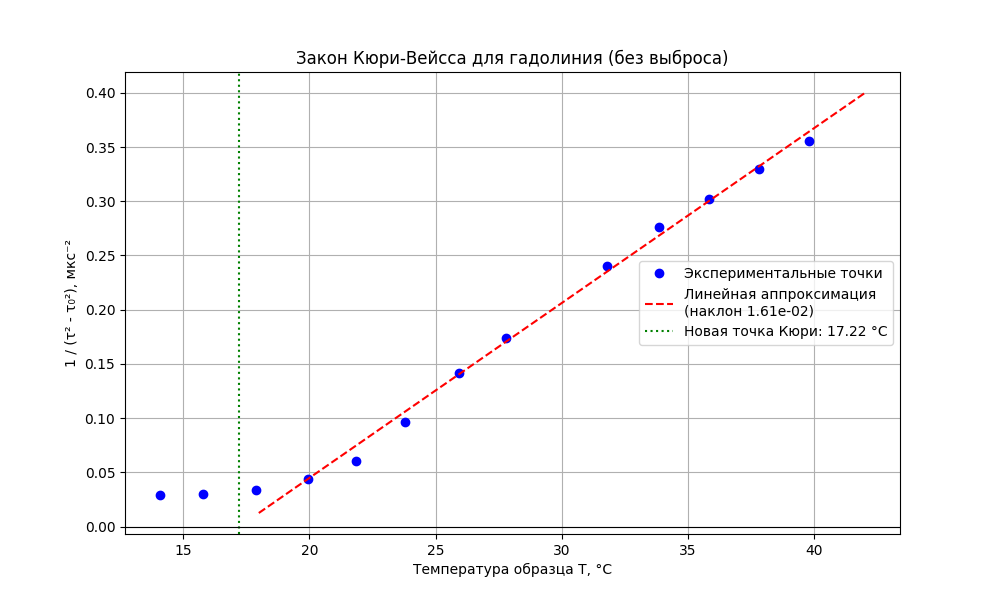
\includegraphics[width=1\textwidth]{график2.png}
\caption{Зависимость обратной величины магнитной восприимчивости от температуры (без учета выброса)}
\label{fig:graph_filtered}
\end{figure}

Аппроксимируя линейный участок графика (для температур \(T > 22^\circ\text{C}\)), экстраполируем полученную прямую к оси абсцисс. Точка пересечения дает уточненное значение \textbf{парамагнитной точки Кюри}:
\[
\Theta_p \approx 17.2 ^\circ\text{C}.
\]

По участку, отклоняющемуся от линейной зависимости (при \(T < 20^\circ\text{C}\)), оценим положение \textbf{ферромагнитной точки Кюри} \(\Theta_K\). Отклонение от закона Кюри--Вейсса начинается примерно при \(T \approx 20 \dots 21 ^\circ\text{C}\), что соответствует \(\Theta_K \approx 20.5 ^\circ\text{C}\) и хорошо согласуется с табличным значением для гадолиния (\(\approx 20^\circ\text{C}\)).






\section{Вывод}
В ходе работы была исследована температурная зависимость магнитной восприимчивости гадолиния выше точки Кюри. Установлено, что в парамагнитной области (при \(T > 22^\circ\text{C}\)) выполняется закон Кюри--Вейсса: обратная величина магнитной восприимчивости линейно зависит от температуры.

В процессе обработки экспериментальных данных была выявлена аномальная точка при \(30^\circ\text{C}\). Данная точка была исключена из рассмотрения как грубый промах. 

После исключения выброса линейная аппроксимация графика в координатах \(1/(\tau^2 - \tau_0^2)\) от \(T\) позволила путем экстраполяции к оси абсцисс определить парамагнитную точку Кюри:
\[
\Theta_p \approx 17.2^\circ\text{C}.
\]
По началу отклонения экспериментальных точек от линейной зависимости была оценена ферромагнитная точка Кюри:
\[
\Theta_K \approx 20.5^\circ\text{C}.
\]

Полученные значения хорошо согласуются с табличными данными для гадолиния (\(\Theta_K \approx 20^\circ\text{C}\)), что подтверждает применимость закона Кюри--Вейсса для описания парамагнитного состояния ферромагнетиков при температурах выше точки фазового перехода.









\end{document}
